\documentclass[twoside,floatfix,a4wide]{revtex4}
\usepackage{multirow} % common packages
\usepackage{url}
\usepackage{hyperref}
\usepackage{listings}
\usepackage{graphicx}
\usepackage{fancyhdr}
%\usepackage{asymptote}
%\usepackage{amsmath}
\usepackage{color}
\definecolor{mydarkred}{rgb}{0.7,0,0}
\newcommand{\checkme}[1] {\textcolor{mydarkred}{{\bf CHECK ME:}  \{#1\}}}
\newcommand{\comment}[1] {\textcolor{mydarkred}{\em  \{#1\}}} 

%\numberwithin{equation}{section} % Eguation numbering with section id. Reguires amsmath -package.
\pagestyle{fancy}
\fancyhead{} % clear all fields

\fancyhead[L]{\bf {January 19, 2008}} % Left Odd, Right Even
\fancyfoot[L]{A.~Heikkinen {\em et al.}: 
{\em Ideal $\tau$ tagging with TMVA multivariate data-analysis toolkit}}

\fancyhead[R]{\thepage}
\fancyfoot[C]{} 
\newcommand{\urltilde}[1]{\texttt{#1}} % solves the tilde problem

\bibliographystyle{apsrev}

\hypersetup{
    bookmarks=true,         % show bookmarks bar?
    unicode=false,          % non-Latin characters in Acrobat’s bookmarks
    pdftoolbar=true,        % show Acrobat’s toolbar?
    pdfmenubar=true,        % show Acrobat’s menu?
    pdffitwindow=true,      % page fit to window when opened
    pdftitle={My title},    % title
    pdfauthor={Author},     % author
    pdfsubject={Subject},   % subject of the document
    pdfnewwindow=true,      % links in new window
    pdfkeywords={keywords}, % list of keywords
    colorlinks=true,        % false: boxed links; true: colored links
    linkcolor=red,          % color of internal links
    citecolor=green,        % color of links to bibliography
    filecolor=blue,         % color of file links
    urlcolor=red            % color of external links
}

\begin{document}

\title{Ideal $\tau$ tagging with TMVA multivariate data-analysis toolkit
\footnote{Paper \cite{ah09bProceedings} in preparation for CHEP 2009, 21 - 27 March 2009 Prague, 
Czech Republic}}
%\url{http://www.particle.cz/conferences/chep2009/}}
%\title{A Geant4 physics list for spallation reactions}

\author{\underline{A.~Heikkinen}, P.~Kaitaniemi, V. Karim\"{a}ki,
 R.~Kinnunen,  M.~J.~Kortelainen, T.~Lamp\'{e}n, S.~Lehti, T.~Lind\'{e}n, and L.~Wendland} 
\affiliation{Helsinki Institute of Physics, P.O. Box 64, FIN-00014 University of Helsinki, Finland.
E-mail: aatos.heikkinen@cern.ch}

\begin{abstract}
We report our experience on using ROOT package TMVA for
multivariate data analysis, for a problem of $\tau$ tagging in the
framework of heavy charged MSSM Higgs boson searches at the LHC.
With a generator level analysis, 
we investigate how in the ideal case $\tau$ tagging could be performed and 
hadronic $\tau$ decays separated from the
hadronic jets of QCD multi-jet background present in LHC experiments. 
A successful separation of the Higgs signal from the background 
requires a rejection factor of $10^5$ or better against the QCD background. 
The $\tau$ tagging efficiency and background rejection are studied with various MVA classifiers.

%{\bf CHEP'07 abtract (see \cite{heikkinen07lProceedings}):}
%{\em We test the usage of a Toolkit for Multivariate Data Analysis (TMVA) in b tagging.
%Tagging b jets associated with heavy neutral MSSM Higgs bosons at the LHC can be used to
%extract the Higgs bosons from the Drell-Yan background, for which the associated jets are
%mainly light quark and gluon jets. Achievable b tagging effciency is studied with more than
%ten MVA classifiers at 1% mistagging rate. Most classifiers were found to perform better than
%the simple track counting 

\end{abstract}

\maketitle


\tableofcontents

\thispagestyle{fancy}

\section{INTRODUCTION \label{section:intro}}
We have previously tested TMVA software in b-tagging for the search of MSSM Higgs bosons 
at the LHC \cite{heikkinen07lProceedings}.
\section{MULTIVARIATE DATA ANALYSIS}
\subsection{TMVA methodology}


\section{DATA AND VARIABLES}
\subsection{Event generation}
\subsection{Ideal case vs. detector effects}
% smearing
\subsection{Discriminating variables}


\subsection{IMPLEMENTATION \label{section:implementation}}
[code example]

[listing waht was coded, changed in TMVA]

\section{RESULTS} \label{sec:example}
\subsection{[Aatos] NN analysis}

{\tt root\_v5.21.06}
Compiled with {\tt make -j2} option used for dual CPU machines.

\scriptsize
\begin{verbatim}

\end{verbatim}
\normalsize

\scriptsize
\begin{verbatim}
\end{verbatim}
\normalsize

\scriptsize
\begin{verbatim}

\end{verbatim}
\normalsize


\scriptsize
\begin{verbatim}
\end{verbatim}
\normalsize

\subsubsection{Default variables, default cuts}
\scriptsize
\begin{verbatim}

\end{verbatim}
\normalsize

(See Figs.\ref{fig:variables_c1}),
 
\begin{figure}[h]
 \begin{minipage}{7.0cm}
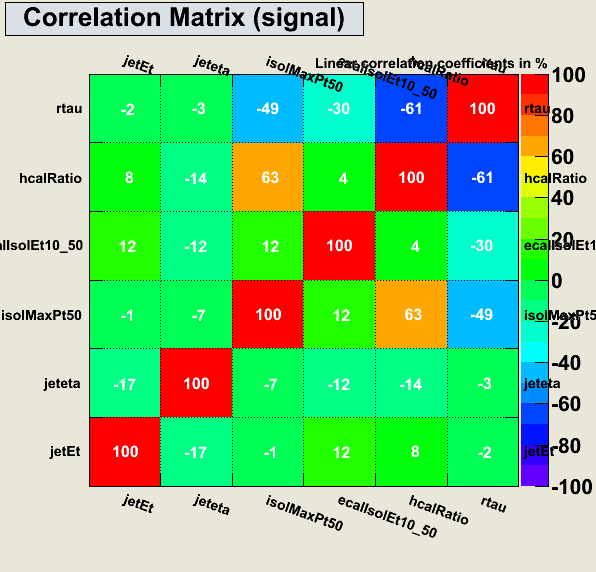
\includegraphics[width=1.0\textwidth]{images/ahCorrelationMatrixS.png}
\end{minipage}
 \hfill
\begin{minipage}{7.0cm}
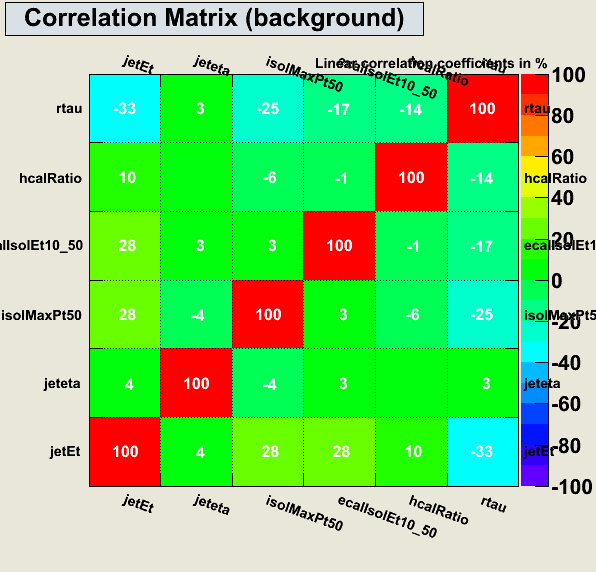
\includegraphics[width=1.0\textwidth]{images/ahCorrelationMatrixB.png}
\end{minipage}
\begin{minipage}{3.0cm}
\caption{Right: Variable correlation matrix for signal Right: Variable correlation matrix for background}
\end{minipage}
\label{fig:ahCorrelationMatrix}
\end{figure}


\begin{figure}[h]
\begin{center}
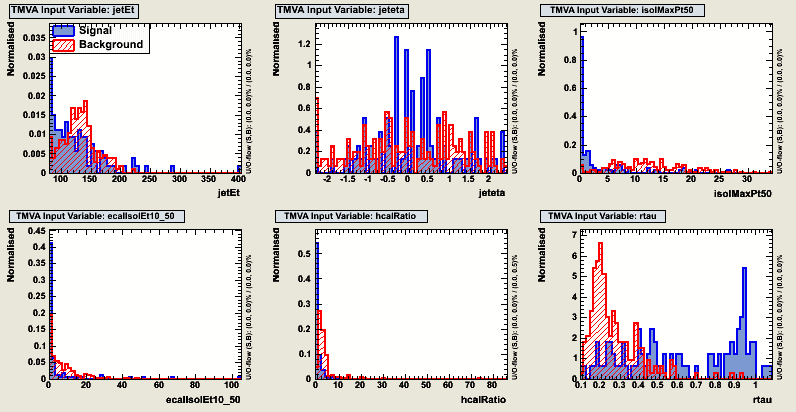
\includegraphics[width=1.0\textwidth]{images/ahVariables_c1.png}
\caption{Variables used in the analysis. Notice log transformations used for some of the variables.}
\label{fig:variables_c1}
\end{center}
\end{figure}

 
\begin{figure}[h]
 \begin{minipage}{7.0cm}
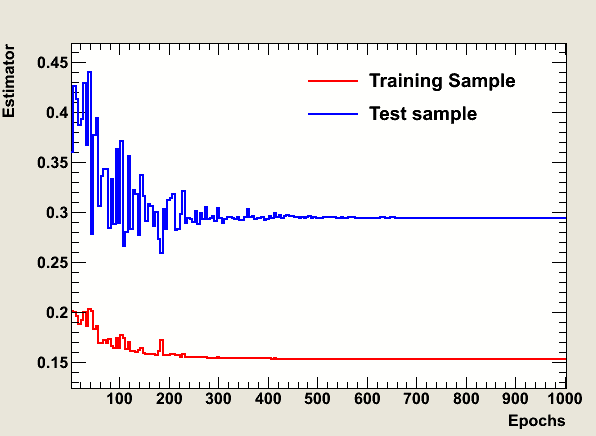
\includegraphics[width=1.0\textwidth]{images/ahAnnconvergencetest.png}
\end{minipage}
 \hfill
\begin{minipage}{7.0cm}
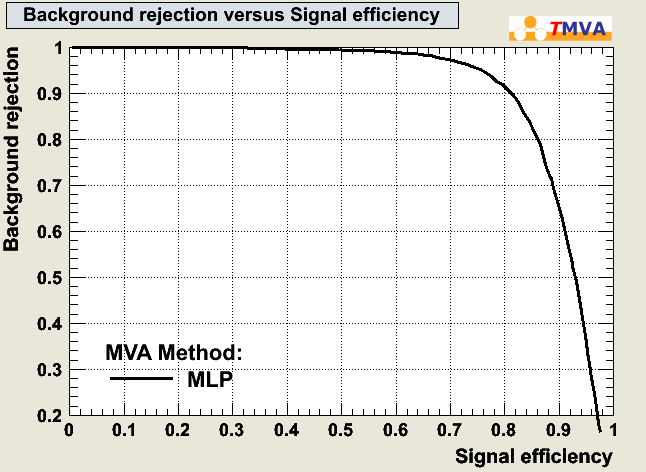
\includegraphics[width=1.0\textwidth]{images/ahRejBvsS.png}
\end{minipage}
\begin{minipage}{3.0cm}
\caption{Left: ANN convergence test. Right: Signal vs. background rejection for ANN classifier.}
\end{minipage}
\label{fig:mlp}
\end{figure}


\clearpage

\begin{figure}[!h]
\begin{center}
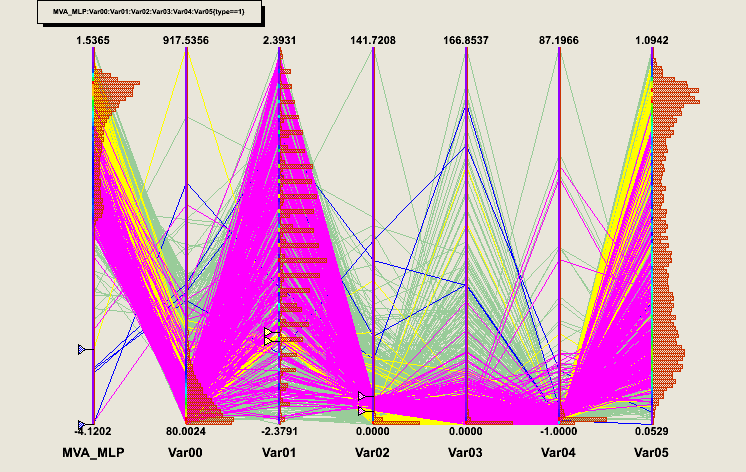
\includegraphics[width=0.6\textwidth]{images/ahParacoor_c0_S.png}
\caption{Parallel coordinates for signal. 
(For more information on parallel coordinates plot see \url{http://en.wikipedia.org/wiki/Parallel_coordinates}.)}
\label{fig:ahParacoor_c0_S}
\end{center}
\end{figure}
\begin{figure}[!h]
\begin{center}
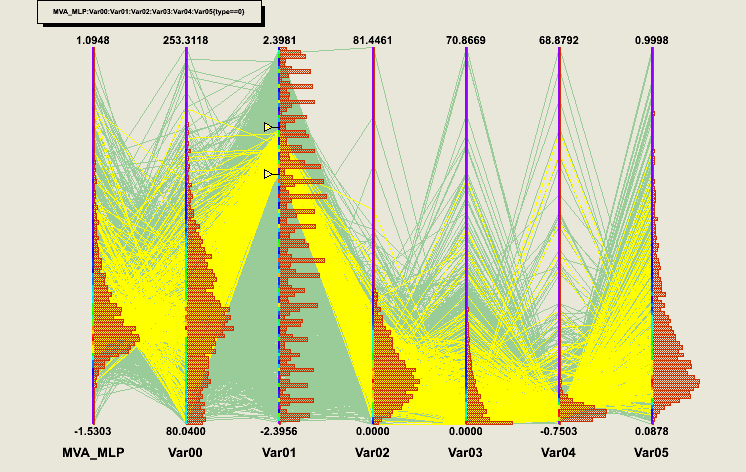
\includegraphics[width=0.6\textwidth]{images/ahParacoor_c0_B.png}
\caption{Parallel coordinates for background}
\label{fig:ahParacoor_c0_B}
\end{center}
\end{figure}

\clearpage

 
\begin{figure}[h]
 \begin{minipage}{7.0cm}
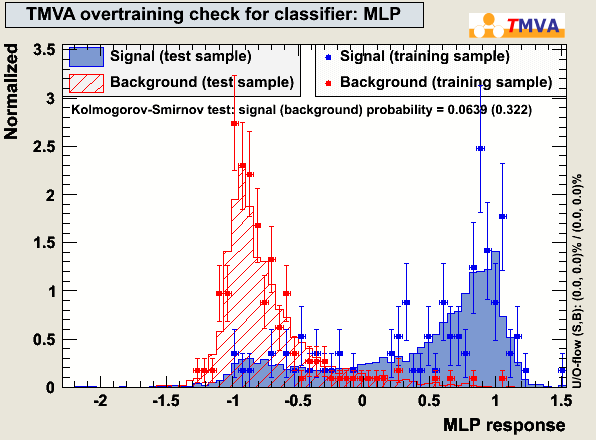
\includegraphics[width=1.0\textwidth]{images/ahOvertrain_MLP.png}
\end{minipage}
\hfill
\begin{minipage}{7.0cm}
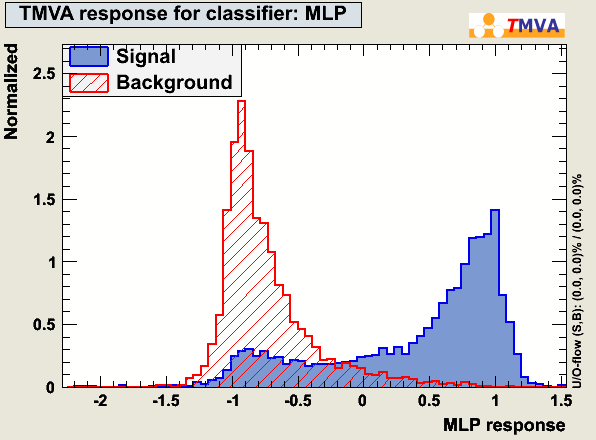
\includegraphics[width=1.0\textwidth]{images/ahMva_MLP.png}
\end{minipage}
\begin{minipage}{3.0cm}
\scriptsize
\caption{Left: Overtrain test. Right: MLP output for test data.}
\normalsize
\end{minipage}
\label{fig:mlp}
\end{figure}



%\subsection{chep09tmva\_aatos.C}
\lstset{
language=C++,
numbers=left,
stepnumber=2,
caption={\tt code/chep09tmva\_aatos.C},
label=chep09tmva_aatos
}
%\lstinputlisting{code/chep09tmva_aatos.C}

%\subsection{chep09tmva.cc}
\lstset{
language=C++,
numbers=left,
stepnumber=2,
caption={\tt code/chep09tmva.cc},
label=chep09tmvacc
}
%\lstinputlisting{code/chep09tmva.cc}


%git fetch pekka
%git merge pekka/master
%gitk 
%(modify)
%git diff
%git status
%git commit -a -m 'comment'  (add all changes)
%(modify)
%git diff
%git commit -a -m 'comment'  

%gitk 
%git revert HEAD  (in case of bad commit this reverses it)

%git push 

%make release



%.gitconfig}:
%
%[user]
%	email = aatos.heikkinen@cern.ch
%[color]
%       ui = auto






 % NN
\subsection{Function discriminant analysis, FDA}

\begin{figure}[h]
\begin{center}
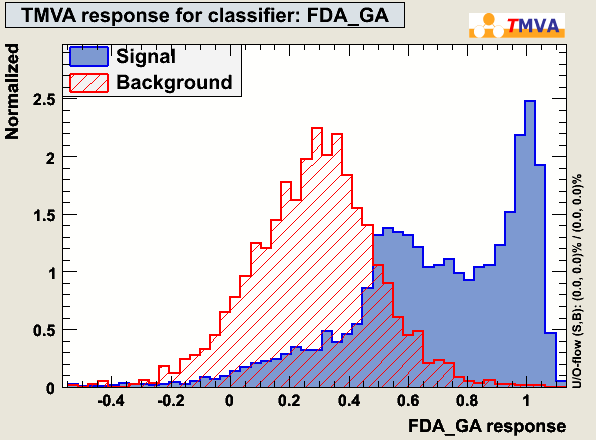
\includegraphics[width=1.0\textwidth]{images/pkMva_FDA_GA.png}
\caption{mvaFDA using genetic algorighm (GA)}
\label{fig:pkMvaFDAGA}
\end{center}
\end{figure}

\begin{figure}[h]
\begin{center}
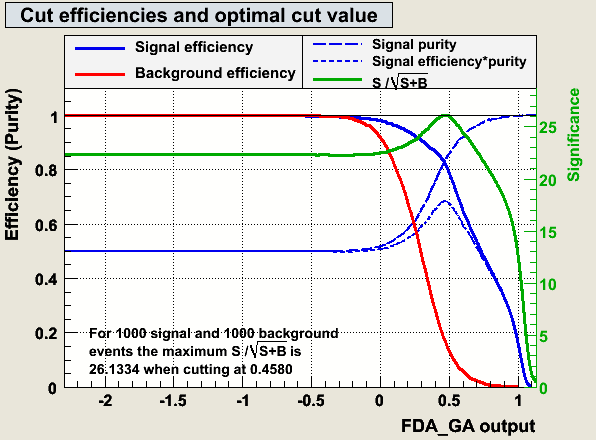
\includegraphics[width=1.0\textwidth]{images/pkMvaEffs_FDA_GA.png}
\caption{FDA GA }
\label{fig:pkMvaEffsFDAGA}
\end{center}
\end{figure}

\begin{figure}[h]
\begin{center}
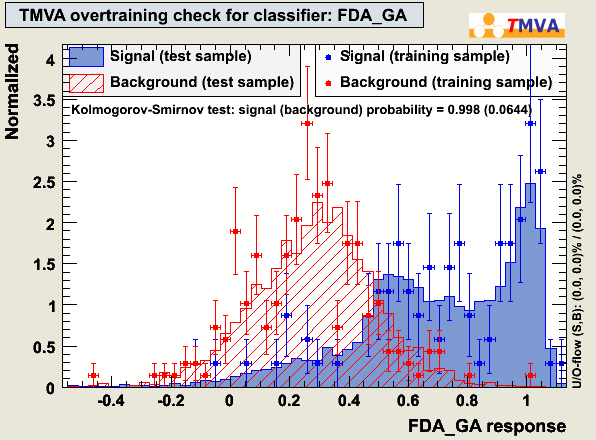
\includegraphics[width=1.0\textwidth]{images/pkOvertrain_FDA_GA.png}
\caption{FDA GA }
\label{fig:pkOvertrainFDAGA}
\end{center}
\end{figure}


\subsection{k-nearest neighbour method, kNN}

\begin{figure}[h]
\begin{center}
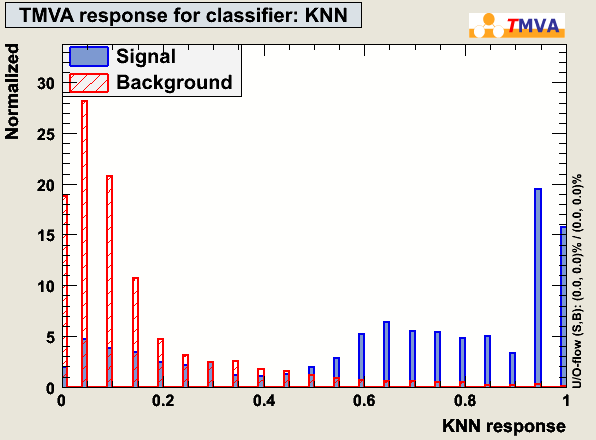
\includegraphics[width=1.0\textwidth]{images/pkMva_KNN.png}
\caption{MVAKNN}
\label{fig:pkMvaKNN}
\end{center}
\end{figure}

\begin{figure}[h]
\begin{center}
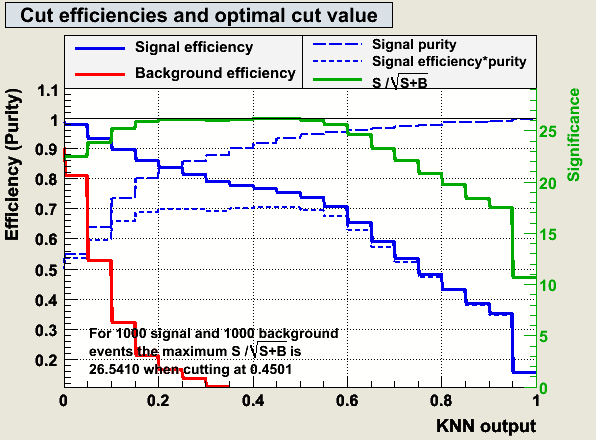
\includegraphics[width=1.0\textwidth]{images/pkMvaEffs_KNN.png}
\caption{KNN}
\label{fig:pkMvaEffsKNN}
\end{center}
\end{figure}

\begin{figure}[h]
\begin{center}
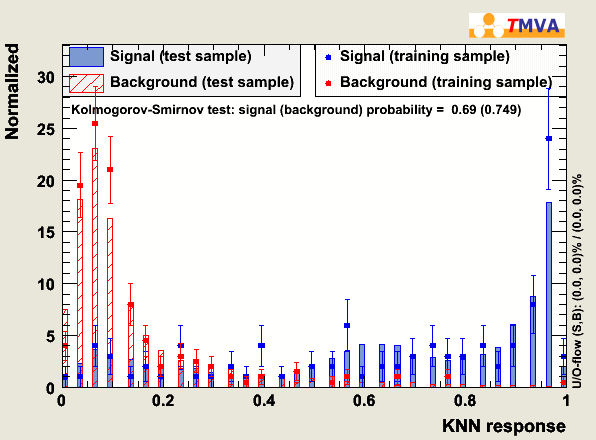
\includegraphics[width=1.0\textwidth]{images/pkOvertrain_KNN.png}
\caption{KNN}
\label{fig:pkOvertrainKNN}
\end{center}
\end{figure}

\begin{figure}[h]
\begin{center}
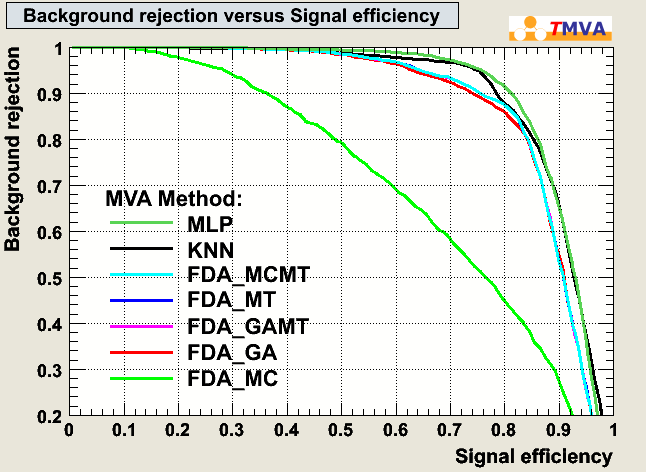
\includegraphics[width=1.0\textwidth]{images/pkRejBvsS.png}
\caption{ROC curve (MLP added as a benchmark)}
\label{fig:pkRejBvsS}
\end{center}
\end{figure}

\clearpage

\subsection{[VEIKKO]}
\subsection{[RITVA]}
\subsection{[Matti] SVM}

\subsubsection{General notes}
\begin{itemize}
\item Number of bins for the ROC curve is 100, and specified in
  \texttt{src/Config.cxx} under the TMVA source tree.
  \begin{itemize}
  \item This can be changed by \texttt{TMVA::gConfig().GetVariablePlotting().fNbinsXOfROCCurve = 1000;}
  \item It looks like when the ROC curve is constructed (in
    \texttt{src/MethodBase.cxx}; except for Cuts), the background
    efficiency is interpolated with splines from a histogram with
    $10^4$ bins. The histogram in question is the bacgkround
    efficiency as a function of discriminator value
  \item It could be possible to recompute the ROC curve in a plotting
    script (except for Cuts)
  \item The whole thing is probably not a problem, since the
    background efficiency is floating point number
  \end{itemize}
%\item All variables (branches) in the tree are float, right? \textbf{Yes}
\item Signal and background event weights are now both 1. This should
  probably be fixed; is hardcoding to \texttt{code/chep09tmva} ok or
  do we want it to be a configuration parameter?
\item The normalization mode should be checked(NormMode parameter for
  the trainer, currently it has the value NumEvents), also the
  SplitMode (now Random) might not be good
%\item In the case that the big data is in madhatter, we should use
%  ametisti (or sepeli). I think we should at least discuss about the
%  possibility of having the data in ametisti instead of madhatter.
\item The \texttt{TestTree} tree in output \texttt{TMVA.root} can be
  used to see the output distributions of the variables after placing
  a cut on the classifier discriminator
  \begin{itemize}
  \item The branch \texttt{type} seems to be 0 for background and 1 for signal
  \end{itemize}
\item What number(s) should we look when optimizing the classifier?
  \begin{itemize}
  \item Signal efficiency at $10^5$ background rejection?
  \end{itemize}
\item What to do with the random number seed problem we had last time?
  \begin{itemize}
  \item The training of some classifiers depends highly on the random
    number generator(s). There is really no global random number seed,
    so the training might be in general indeterministic with respect
    to the parameters of the classifier.
  \item Few options comes to my mind:
    \begin{itemize}
    \item[a)] Try to look the average training behaviour by training
      several classifiers with same parameters by (somehow) varying
      the random number seed.
    \item[b)] Choose the parameters with which the classifier
      performance is best
    \end{itemize}
  \end{itemize}
\item It seems that the Cuts classifier evaluation time scales
  quadratically w.r.t the size of the test tree. (Our event evalution
  with \texttt{MyEvaluate} has linear scaling.)% This behaviour is
  %demonstrated in table~\ref{table:mkCutsScaling} and in
  %figure~\ref{fig:mkCutsScaling}.
  Other classifiers might not be incluenced by this, as is
  demonstrated in the table with SVM.

  \textbf{Update 2009-02-05:} This seems to be affected also by the
  (background) data. When the jets with $\texttt{jeteta}=0$ are
  removed, Cuts classifier gets evaluated also in reasonable time
  (faster than in \texttt{MyEvaluate}).
\end{itemize}

% \begin{table}
%   \caption{Comparison of TMVA evaluation to our event
%     testing+evaluation with Cuts and SVM classifiers. The numbers are
%     real time in seconds, and they are \textbf{suggestive only}.}
%   \label{table:mkCutsScaling}
%   \begin{center}
%     \begin{tabular}{c|cc|cc}
%       Training & \multicolumn{2}{|c|}{Cuts} & \multicolumn{2}{|c}{SVM} \\
%       jets     & TMVA test+eval. & Event eval.   & TMVA test+eval. & Event eval. \\
%       \hline
%       10000    & 0.43            & 1.13          & 0.67            & 0.73 \\
%       20000    & 1.53            & 1.75          & 1.21            & 1.53 \\
%       50000    & 12.1            & 4.04          & 2.15            & 2.03 \\
%       80000    & 32.6            & 6.19          & 2.70            & 2.81 \\
%       100000   & 51.1            & 7.55          & 3.84            & 3.26 \\
%       150000   & 114             & 11.3          & 5.70            & 6.36 \\
%       200000   & 202             & 15.4          & 7.42            & 6.00 \\
%       250000   & 315             & 18.6          & 7.99            & 8.36 \\
%       300000   & 440             & 22.4          & 11.1            & 10.2 \\
%       400000   & 893             & 29.9          & 12.4            & 11.5 \\
%       500000   & 1560            & 38.8          & 18.3            & 16.2
%     \end{tabular}
%   \end{center}
% \end{table}

% \begin{figure}
%   \begin{center}
%     \begin{minipage}{.35\textwidth}
%       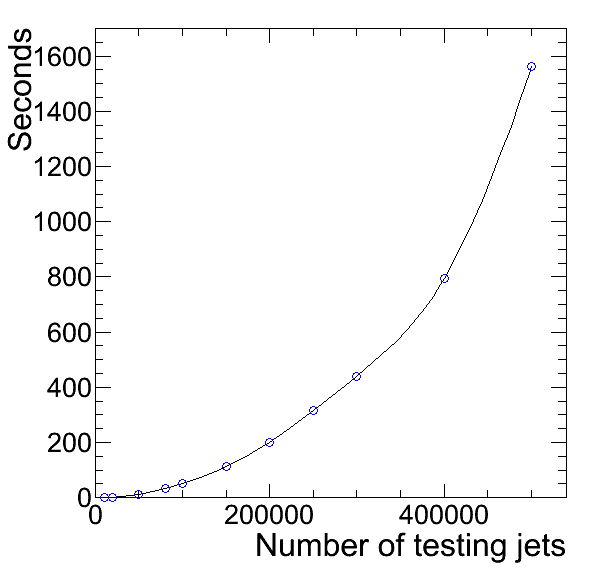
\includegraphics[width=\textwidth]{images/mkTmvaEval}
%     \end{minipage}
%     \hspace{.1\textwidth}
%     \begin{minipage}{.35\textwidth}
%       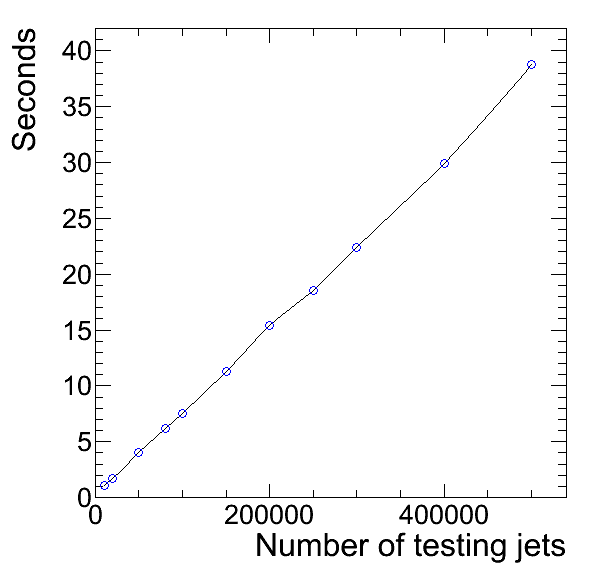
\includegraphics[width=\textwidth]{images/mkEventEval}
%     \end{minipage}
%   \end{center}
%   \caption{Real time spent in TMVA testing and evaluation together
%     (left) and in our event evaluation (right) as a function of
%     testing jets in input for Cuts classifier. The plots are
%     \textbf{suggestive only}, because they were produced from a single
%     run per data point and the reported time is real time.}
%   \label{fig:mkCutsScaling}
% \end{figure}


\subsubsection{Jet vs. event efficiencies}

\begin{itemize}
\item The input \texttt{TTree} for TMVA has jets as entries (i.e. TMVA
  ``event'' corresponds to a jet in the event generated in Pythia), so
  the efficiencies (and other quantities) reported by TMVA are for
  jets. The tree has branches for event and run numbers, so it is
  possible to separate the jets belonging to different events.
\item In the end, in order to have a physically reasonable result and
  to compare with other results, we would like to have the
  signal/background efficiencies of events, not jets (e.g. event is
  passed if there is at least one jet passing the classifier,
  otherwise the event is rejected)
\item In order to ``convert'' the jet efficiencies to event
  efficiencies, some kind of counting must be done
  \begin{enumerate}
  \item[a)] Optimisation is done only with jets, and for the final
    results the classifiers are used in event basis. Our abstract
    doesn't clearly specify, what we mean by $10^5$ background
    rejection (event vs. jet rejection).

  \item[b)] Use TMVA training tree for re-counting. However, the
    training tree contains only the variables used for training, and
    classifier outputs for the corresponding jets. In the current TMVA
    (v3.9.x) it seems to be impossible to add variables, which are not
    used for training/testing, to the training tree.

    It is of course possible to take the standalone TMVA as a part of
    our package and include this functionality. Actually, this has
    been requested in the TMVA users mailing list in 2007
    (\url{http://sourceforge.net/mailarchive/forum.php?thread_name=471C8D74.6040209\%40mpi-hd.mpg.de\&forum_name=tmva-users}),
    and it is in the TODO list
    (\url{http://tmva.cvs.sourceforge.net/tmva/TMVA/development/todo.txt?view=markup})
    with \emph{high priority}. Thus, my motivation of implementing
    this feature is not so high.

  \item[c)] Use the TMVA input tree for performing our own event-based
    counting. The TMVA preselection cuts and variable transformations
    will cause some headache, but it could be manageable. It might be
    easiest to take relevant pieces of code from TMVA and add glue,
    tape and gum to make it work. In order to not to use training data
    for testing, the training and testing trees should be in different
    files.
  \end{enumerate}
\item Currently (after commit
  82e7bc3d9575e853df7b65ebbbcdf5d91232802d) the event efficiencies are
  evaluated with the approach c). There are few things which should be
  noted in the current implementation
  \begin{description}
  \item[Training/test tree] The information about which jets are used
    for training by TMVA is not available (at least easily). Therefore
    the whole input tree is processed. This means, that if the one
    tree (or chain) is used for both training and testing in TMVA, the
    results produced by our evaluation code are biased. Fortunately, I
    think Lauri agreed about having the training and testing data in
    separate files (i.e. chains).

    The current code already supports separate chains for training and
    testing. If only training chain is defined (i.e. testing chain is
    empty), the training chain is used for both training and testing,
    as the situation was before.

  \item[Cuts vs. others] The signal/background efficiencies for other
    classifiers than cuts are produced with a code similar to the
    related code in TMVA, with the exception that only one jet per
    event is counted. However, Cuts classifier is a different story.

    The Cuts classifier is trained such that for each signal
    efficiency bin of ROC curve, TMVA maximizes the the background
    rejection. As some of the optimization algorithms have stochastic
    nature, the resulting ROC curve can have peaks. This means that
    for a given background efficiency level there might be multiple
    signal efficiencies (with different set of cuts, of course). TMVA
    chooses the smallest signal efficiency for their output, I've
    chosen the greatest (this also applies to other classifiers than
    Cuts, but for them I'd expect that ROC is smooth).

    Another difference comes from the fact that when other classifiers
    return a number which correlates with the probabability of the jet
    being $\tau$ jet, Cuts classifier returns boolean true/false
    (corresponding to a given signal efficiency). In order to test all
    trained cuts, all training signal efficiencies are looped over,
    and the TMVA reader is asked if the jet in question passes the
    cut. The number of passed events for each training signal
    efficiency is recorded, and with these \emph{true} signal and
    background efficiencies the ROC curve is constructed. The points
    with zero signal efficiency are not used, as they're probably just
    cases where the training has failed.

  \item[Reporting in output] The output of \texttt{chep09tmva} program
    became large, and it was also requested that it would be possible
    to switch \texttt{MyEvaluate} off. I added
    \texttt{AdditionalReports} section to the configuration file,
    where the possible reports can be switched on/off by
    (un)commenting the corresponding line. In the default
    configuration of \texttt{tmva-common.conf} and
    \texttt{tmva-example.conf} all reports are enabled.

  \item[Integration with TMVAGui.C?] Signal/background event
    efficiency histograms as well as the resulting ROC curves are
    stored to the output ROOT file. This enables the possibility to
    add these plots to the \texttt{TMVAGui.C} script.

    It should be noted that all other plots are histograms
    (\texttt{TH1}) except the ROC for Cuts, which is \texttt{TGraph}.

  \item[Maximum number of testing entries] \texttt{MyEvaluate} uses
    the same configuration as TMVA Factory (i.e. \texttt{NSigTest} and
    \texttt{NBkgTest} under \texttt{Trainer}) for specifying the
    maximum number of entries used for testing. If these are zero, all
    entries are used. It should be noted that unless both TMVA and
    \texttt{MyEvaluate} process the test trees entirely, they might
    process different entries.

  \item[Error estimation] Currently the reported errors come from the
    formula $\sigma=\sqrt{\varepsilon(1-\varepsilon)/N}$ as in TMVA.
    Should we also try to take the effect of binning into account?

  \end{description}
\end{itemize}

\subsubsection{SVM Notes}
%% \begin{itemize}
%% \item Training time scales as $O(n^2)$ where $n$ is the size of the
%%   input data (i.e. number of events)
%%   \begin{itemize}
%%   \item 100 signal and 200 background events took 0.125 seconds
%%   \item 200 signal and 400 background events took 0.542 seconds
%%   \item 500 signal and 1000 background events took 3.41 seconds
%%   \item 800 signal and 1600 background events took 10 seconds
%%   \item 1000 signal and 2000 background events took 13.8 seconds
%%   \item If the scaling law is correct, $10^4$ events would take about 2
%%     minutes, $5\times 10^4$ events would take almost an hour and $10^5$
%%     events would take more than 3,5 hours.
%%   \end{itemize}
%% \end{itemize}

\begin{itemize}
\item So far the best achieved signal event efficiency is $5.2\;\%$
  with parameters $\textrm{sigma}=4, \textrm{C}=7$.
\item The parameters for the best signal jet efficiency are
  $\textrm{sigma}=3,\textrm{C}=9$, which gives for event efficiency
  $4.6\;\%$. This shows that there is a difference between
  optimisation of jet and event efficiencies.
\end{itemize}

\subsubsection{TMVA Comments}
\begin{itemize}
\item The ROC curve for Cuts classifier is probably inconsistent with
  the other classifiers. I guess that the signal efficiency comes from
  \textbf{training} and not from testing. For other classifiers the
  signal efficiency comes from testing.
  \begin{itemize}
  \item I created a set of figures (\ref{fig:mkCutsTmva},
    \ref{fig:mkCutsEvalRoc}, \ref{fig:mkCutsEvalEff}) to demonstrate
      this.
  \item The ROC curve from TMVA is in Fig.~\ref{fig:mkCutsTmva}, and
    the ROC curve by the custom evaluator is in
    Fig.~\ref{fig:mkCutsEvalRoc} (the evaluator was modified to
    evaluate jets instead of events for this particular exercise). A
    few things can be seen.
    \begin{itemize}
    \item For some signal efficiency bins, TMVA reports zero for
      backgound efficiency (more or less correct), but one for
      background rejection (can \emph{not} be correct!)
    \item There's also some difference in the signal efficiencies
      (i.e. the $x$-axes of the figues)
    \end{itemize}
  \item Fig.~\ref{fig:mkCutsEvalEff} shows the evaluated background
    and signal jet efficiencies as a function of the \emph{requested}
    signal efficiency (i.e. the parameter given to the
    \texttt{TMVA::Reader} for Cuts classifier).
    \begin{itemize}
    \item For some signal efficiency bins the trained Cuts classifiers
      don't pass any signal/background jets.
    \item The difference between the evaluated signal efficiency and
      the requested signal efficiency is clear.
    \end{itemize}
  \end{itemize}

\item In the case of Cuts, the background rejection could be wrong.
  E.g. it might happen that the cuts optimisation fails for some
  (training) signal efficiency or otherwise the cut values are
  non-valid. If this kind of cut is then applied to both signal and
  background data, nothing would be accepted, but in the ROC curve
  there is a rejection of 1 in the corresponding (training) signal
  efficiency bin.

\item There are a few special cases where the \emph{signal efficiency
    at bkg eff} numbers in the stdout could be wrong
  \begin{itemize}
  \item The achieved bacgkround efficiency is greater/smaller
    \emph{for all} signal efficiencies than the requested bkg eff
  \end{itemize}
\end{itemize}

\begin{figure}[h]
  \begin{center}
    \begin{minipage}{.3\textwidth}
      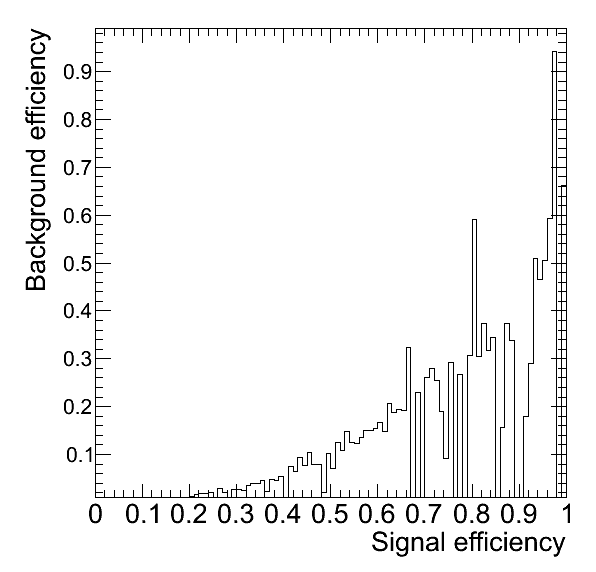
\includegraphics[width=\textwidth]{images/mk_cuts-tmva-effBvsS}
    \end{minipage}
    \hspace{.02\textwidth}
    \begin{minipage}{.3\textwidth}
      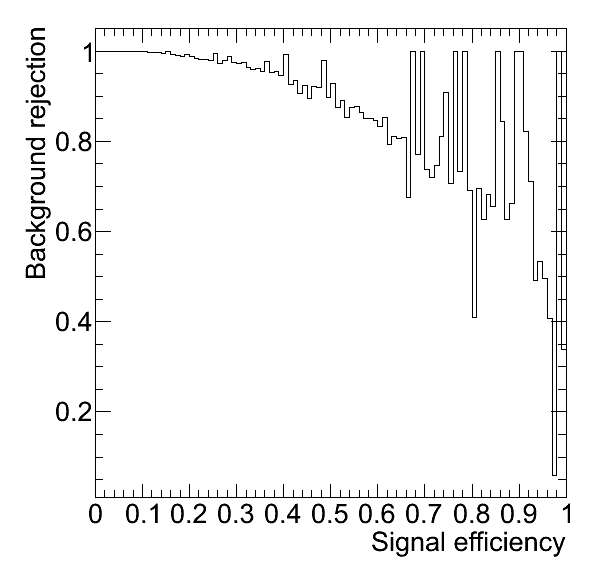
\includegraphics[width=\textwidth]{images/mk_cuts-tmva-rejBvsS}
    \end{minipage}
  \end{center}
  \caption{Background jet efficiency (left) and rejection (right)
    function of signal jet efficiency as reported by TMVA. At high
    signal efficiency there are some points where the background
    efficiency (rejection) is zero (one) because the training of the
    Cuts classifier for those signal efficiencies has produced a cut
    ensemble which doesn't pass any jet.}
  \label{fig:mkCutsTmva}
\end{figure}

\begin{figure}[h]
  \begin{center}
    \begin{minipage}{.3\textwidth}
      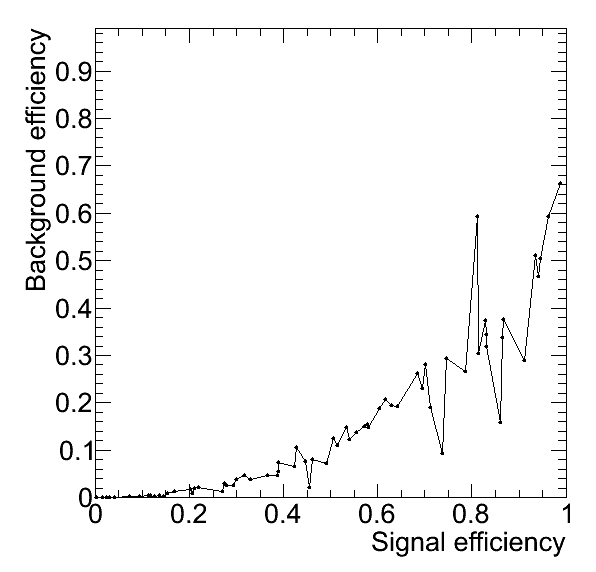
\includegraphics[width=\textwidth]{images/mk_cuts-eval-effBvsS}
    \end{minipage}
    \hspace{.02\textwidth}
    \begin{minipage}{.3\textwidth}
      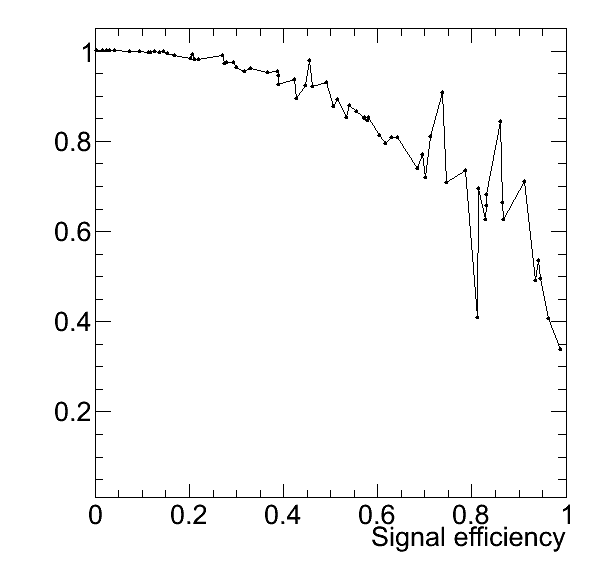
\includegraphics[width=\textwidth]{images/mk_cuts-eval-rejBvsS}
    \end{minipage}
  \end{center}
  \caption{Background jet efficiency (left) and rejection(right) as a
    function of the evaluated signal jet efficiency as reported by our
    custom evaluator. The background and signal efficiencies are the
    efficiencies from the evaluation of all jets. The cases where the
    Cuts classifier doesn't pass any jet were removed from the graphs.}
  \label{fig:mkCutsEvalRoc}
\end{figure}

\begin{figure}[h]
  \begin{center}
    \begin{minipage}{.3\textwidth}
      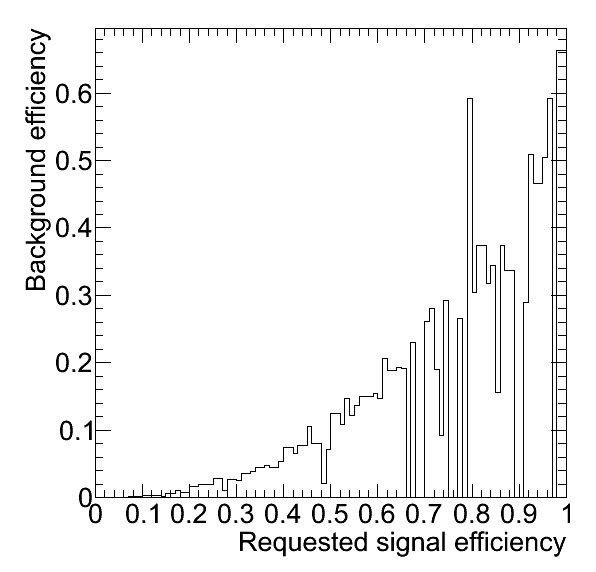
\includegraphics[width=\textwidth]{images/mk_cuts-eval-effB}
    \end{minipage}
    \hspace{.02\textwidth}
    \begin{minipage}{.3\textwidth}
      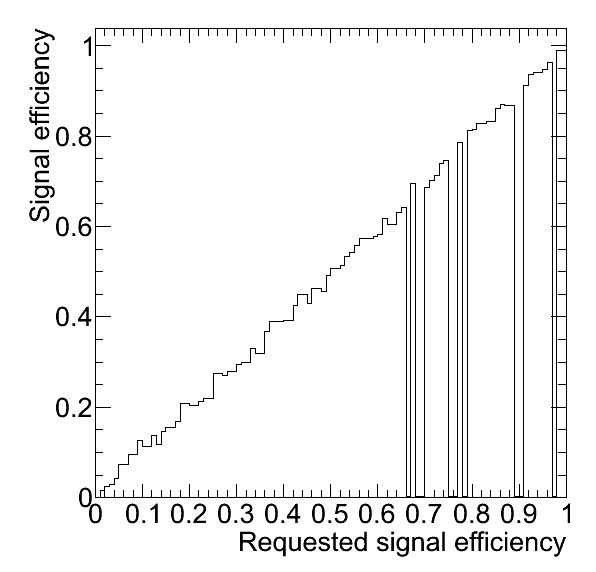
\includegraphics[width=\textwidth]{images/mk_cuts-eval-effS}
    \end{minipage}
  \end{center}
  \caption{Background (left) and signal (right) jet efficiencies as a
    function of the requested signal jet efficiency as reported by our
    custom evaluator. From the signal histogram it can be clearly seen
    that for some requested signal efficiencies none of the jets pass
    the Cuts classifier. It can also be seen that in general the
    achieved signal jet efficiency does not correspond to the
    requested signal jet efficiency.}
  \label{fig:mkCutsEvalEff}
\end{figure}

\clearpage
\subsection{[TAPIO]}
\subsection{[SAMI]}
\subsection{[TOMAS]}
\subsection{[LAURI]}

[Critics: TMVA bugs, is it already mature? Problems?]

[Praisal: what is now working compared to CHEP'07]

\section{CONCLUSION AND DISCUSSION} \label{sec:conclusion}
TMVA

%\begin{lstlisting}
%\end{lstlisting}

\bibliographystyle{unsrt}  % Options plain, unsrt, alpha, abbrv
%\bibliography{refs.bib} %10 p
\bibliography{chep09.bib} %10 p

\begin{appendix}

\lstset{ % General settings
language=c++,                   % choose the language of the code
basicstyle=\ttfamily \small,    % the size of the fonts that are used for the code \footnotsize
numbers=left,                   % where to put the line-numbers
numberstyle=\small,             % the size of the fonts that are used for the line-numbers
stepnumber=2,                   % the step between two line-numbers. If it's 1 each line will be numbered
numbersep=10pt,                 % how far the line-numbers are from the code
showspaces=false,               % show spaces adding particular underscores
showstringspaces=false,         % underline spaces within strings
showtabs=false,                 % show tabs within strings adding particular underscores
frame=,                         % adds a frame around the code (single)
tabsize=2,                      % sets default tabsize to 2 spaces
captionpos=t,                   % sets the caption-position: top (t), bottom (b)
breaklines=true,                % sets automatic line breaking
breakatwhitespace=false,        % sets if automatic breaks should only happen at whitespace
escapeinside={\%*}{*)},         % if you want to add a comment within your code
caption=footnote, 
label=listing:relRef
}

\section{Code}
A code and data will be distributed using git and made abvailable 
at \\ \url{http://www.helsinki.fi/~miheikki/system/refs/heikkinen/ah09bProceedings/code}

\subsection{Makefile}
\lstset{
language=bash,
numbers=left,
stepnumber=2,
caption={\tt code/Makefile},
label=makefile
}
\lstinputlisting{code/Makefile}


\subsection{tmva-common.conf}
\lstset{
language=bash,
numbers=left,
stepnumber=2,
caption={\tt code/tmva-common.conf},
label=tmvacommonconf
}
\lstinputlisting{code/tmva-common.conf}

\subsection{tmva-example.conf}
\lstset{
language=bash,
numbers=left,
stepnumber=2,
caption={\tt code/tmva-example.conf},
label=tmvacommonconf
}
\lstinputlisting{code/tmva-example.conf}

\subsection{ametisti.sh.job}
\lstset{
language=bash,
numbers=left,
stepnumber=2,
caption={\tt code/ametisti.sh.job},
label=ametistishjob
}
\lstinputlisting{code/ametisti.sh.job}

\subsection{chep09tmvaAatos.C}
\lstset{
language=C++,
numbers=left,
stepnumber=2,
caption={\tt code/chep09tmvaAatos.C},
label=chep09tmvac
}
\lstinputlisting{code/chep09tmvaAatos.C}

\subsection{chep09tmva.cc}
\lstset{
language=C++,
numbers=left,
stepnumber=2,
caption={\tt code/chep09tmva.cc},
label=chep09tmvacc
}
\lstinputlisting{code/chep09tmva.cc}

\section{Data files}
Minimalistic example datafile (recommendation: less than 1-2 MB) can
be included in the repository for testing and demonstration
purpooses. Although Git can easily deal with large files, it is
recommended that the production data would not be
included in the repository. It should be kept in mind that GitHub
(and shell accounts) offer relatively limited disk space (GitHub: 100
MB, CERN default: about 150 MB) and that ROOT files can probably not be
compressed further.

For production use it is recommended to store in the repository an URL
to the data. Then we can use the {\tt ROOT} or {\tt HTTP} protocols to
access it or use a {\tt make} directive/shell script to copy the data to the
user's computer. One good example of this practice is the {\tt
HipProofAnalysis} repository. Only the URL:s are stored, not the
data. Additionally also the parameters, configuration options,
software versions, etc. used for the production of the data should
probably be stored in some way in the repository.

\section{WORKING NOTES}
{\bf Suggested  responsibility}: 
\begin{itemize}
\item[aatos]
Aatos: editor, NN classifiers; 
\item Pekka: release manager, git consulting, PROOF
\begin{itemize}
\item git consulting: OK (setting up workflow and repositories, user
  training, documentation, software installation)
\item PROOF: I didn't see PROOF mentioned anywhere in the TMVA
  documentation. Is it supported? If not, then I don't have resources
  to do it (lesson learned in the past: PROOF-enabling an analysis
  code can be a major undertaking...)
\end{itemize}
\item Sami: MC data, 
\item Lauri 1-prog physics
\item Ritva: 
\item Tomas: Ametisti
\item Tapio: 
\item Matti:a mechanism to work with variables 
\item Veikko:
\end{itemize}

\subsection{Code repository}
\begin{itemize}
\item Source code for paper and TMVA script  is available at 
{\tt git://github.com/aatos/chep09tmva.git} (\url{http://github.com/aatos/chep09tmva})
%git commit -a -m 'comment'  (add all changes)
%git push 
%gitk 
\begin{itemize}
\item Pekka:
\begin{verbatim}
git remote add pekka git://github.com/kaitanie/chep09tmva.git

git fetch pekka
git merge pekka/master
make release (inform Pekka where tar.gz is available)
\end{verbatim}

\item Lauri (don't do manually PK as an release manager does this):
\begin{verbatim}
git remote add lauri http://cmsdoc.cern.ch/~wendland/chep09tmva.git

git fetch lauri
git merge lauri/master

\end{verbatim}

\item Matti (don't do manually PK as an release manager does this)::
\begin{verbatim}
git remote add matti git://github.com/makortel/chep09tmva.git

git fetch matti
git merge matti/master
\end{verbatim}
\end{itemize}

\item Alternatively LaTeX-files can be loaded form
\url{http://www.helsinki.fi/~miheikki/system/refs/heikkinen/ah09bProceedings.tar.gz}.

After this you can make your modifications and submit them as a
tarball. The tarball can be created by using command {\tt make
contribution}. The resulting file {\tt chep09tmva-contribution.tar.gz}
can be sent as and e-mail attachment to: {\tt pekka.kaitaniemi@gmail.com}.

\item You can also mail you comments and updates directly to editor (Aatos)
Based on pdf version
\url{http://www.helsinki.fi/~miheikki/system/refs/heikkinen/ah09bProceedings.pdf}.
\end{itemize}

Guide \url{http://ktown.kde.org/~zrusin/git/git-cheat-sheet-medium.png}.

Some git documentation:
\begin{itemize}
\item Git tutorial: \url{http://www.kernel.org/pub/software/scm/git/docs/gittutorial.html}
\item Git with HipProofAnalysis (contains instructions on how to use
  Git on lxplus:
  \url{http://projects.hepforge.org/radical/trac/wiki/GitWithHipProofAnalysis}
\end{itemize}

\subsection{Building the document}

Building the document requires {\tt make} and \LaTeX tools. The
document can be built using the {\tt make} command. At the end of the
compilation this will optionally launch a PDF viewer (by default Firefox browser
and Acrobat Reader plugin). You can change the PDF viewer program by
setting environment variable {\tt PDFVIEWER} to point to your
favourite PDF viewer (e.g. lightweight alternative {\tt xpdf}). To
enable the PDF viewer feature you can set the environment
variable {\tt USEVIEWER} to 1.

\subsection{Current status of TMVA}
For introduction browse, six talks from year 2008 \url{http://tmva.sourceforge.net/talks.shtml}.

\begin{itemize}
\item Current version is TMVA-v3.9.6 (2008, December. 2nd).
\item TMVA (\url{http://tmva.cvs.sourceforge.net}) is now included in ROOT releases:
\begin{itemize}
\item ROOT version 5.22 has been released on December 18, 2008
  (release notes \url{http://root.cern.ch/root/v522/Version522.news.html}),
  it has TMVA-v.3.9.5
\item ROOT version from 5-19-02a to 5-21-01-alice contains TMVA 3.9.4.
\end{itemize}

\item In addition to many bug fixes:
\begin{itemize}
\item Improved prepossessing
\item Pre-selection cuts on arrays. Previously used {\em TEventlists} 
(only event  wise pass/fail) were replaced by {\em TreeFormulas} (sensitive to array position).
\item Plugin capability: custom multivariate classifier can now be plugged into
    the TMVA framework to benefit from TMVA's analysis and performance comparison
    tools. 

\item For details see release notes 
\url{http://tmva.cvs.sourceforge.net/*checkout*/tmva/TMVA/development/RELNOTES}
\end{itemize}

\end{itemize}



\subsection{TMVA run configuration files}

The new example program ({\tt code/chep09tmva.cc}) uses a config file
({\tt code/tmva.conf}) for classifier configuration. There is one
possible problem in this setup. If everyone edits the same file time
and time again, merging everyone's work will become very painful. This
is a problem because we would like people to merge early and
often. There are a few proposals that should be investigated as
possible solutions to this problem:
\begin{enumerate}
\item Using config files is a good option. Hardcoding configs into
the program would probably make merges quite difficult as well.
\item Each user/classifier has a separate config file. The {\tt
chep09tmva} program should have a command line option that allows the
user to choose which configuration is used. An example invocation of
the {\tt chep09tmva} program is shown in listing \ref{configExample}.
\item Ability to have common config options in a separate file
(e.g. {\tt tmva-common.conf}) which could be included into
user/classifier specific configuration files with an {\tt include}
statement. An example of this is shown in listings \ref{commonConfig}
and \ref{userConfig}.
\end{enumerate}

The program has been modified as follows
\begin{itemize}
\item Support for \texttt{include} as shown in listing
  \ref{commonConfig}
\item There is now a common configuration file
  \texttt{tmva-common.conf} (which is still more to demonstrate than
  to really do anything useful), and an example of user configuration
  \texttt{tmva-example.conf}
\item By default it uses the \texttt{tmva-common.conf}, but the
  configuration can be specified as shown in listing \ref{configExample}
  \begin{itemize}
  \item If the same directive (\texttt{Variables:}, \texttt{Cuts:},
    \texttt{Trainer:}, \texttt{Classifiers:}) is given in both the
    user configuration and common configuration, the user
    configuration is used (i.e. e.g. variable lists are not merged).
  \end{itemize}
\end{itemize}



\lstset{
language=bash,
numbers=left,
stepnumber=2,
caption=Example invocation of {\tt chep09tmva} with config file name as a parameter.,
label=configExample
}
\begin{lstlisting}
./chep09tmva pekka.conf
\end{lstlisting}

\lstset{
language=bash,
numbers=left,
stepnumber=2,
caption=Contents of the file {\tt tmva-common.conf} that contains config options shared by all analysis runs.,
label=commonConfig
}
\begin{lstlisting}
// String to pass TMVA::Factory::PrepareTrainingAndTestTree
Trainer:
NSigTrain=1000:NBkgTrain=20000:SplitMode=Random:NormMode=NumEvents:!V
\end{lstlisting}

\lstset{
language=bash,
numbers=left,
stepnumber=2,
caption=Contents of the user specific config file {\tt pekka.conf}.,
label=userConfig
}
\begin{lstlisting}
include tmva-common.conf

Cuts_D H:!V:FitMethod=MC:EffSel:SampleSize=20000:VarProp=FSmart:VarTransform=Decorrelate
\end{lstlisting}

\lstset{ %
language=bash,                % choose the language of the code
basicstyle=\footnotesize,       % the size of the fonts that are used for the code
numbers=left,                   % where to put the line-numbers
numberstyle=\footnotesize,      % the size of the fonts that are used for the line-numbers
stepnumber=2,                   % the step between two line-numbers. 
                                %If it's 1 each line will be numbered
numbersep=5pt,                  % how far the line-numbers are from the code
showspaces=false,               % show spaces adding particular underscores
showstringspaces=false,         % underline spaces within strings
showtabs=false,                 % show tabs within strings adding particular underscores
frame=single,                   % adds a frame around the code
tabsize=2,                      % sets default tabsize to 2 spaces
captionpos=t,                   % sets the caption-position to bottom
breaklines=true,                % sets automatic line breaking
breakatwhitespace=false,        % sets if automatic breaks should only happen at whitespace
escapeinside={\%*}{*)},          % if you want to add a comment within your code
%caption=Bash function to release a directory., 
label=listing:relRef
}

\section{HISTORY}
\begin{itemize}
\item 090113 Release management bug fix.
\item 090112 Testing new release tools developed by our release manager Pekka.
\item 081217 Fixed some lost files by Merging from Pekka.
\item 081216 Merge from Matti and Pekka. 
Files added for each author, corresponding a specific analysis subsection.
First test runs for MLP done using {\tt chep09tmva.C}. Sample images added to {\tt ah09bProceedings.tex}.
\item 081215 This abstract was accepted as CHEP'09 talk.
\item 081202 Merging example data and related configuration file from Lauri.
\item 081125 Merging from Lauri, Matti, and Pekka. 
Added subsections for code listing and table of contents.
\item 081111 Merging branch from Lauri and including comments from Sami. 
Based on discussion at HIP group weekly meeting made some aditional changes to abtract.
\item 081028 Project released in \url{http://github.com/aatos/chep09tmva}. Removed proceedings notes in the Appendix A to separate file {\tt notes.tex}.
\item 091029 PK: Commented some points in the proposed
  responsibilities. Added a couple of links to the Git documentation.
\item 081021 Title and abstract focus improved after discussion in the group. 
\item 081014 First draft done after the idea to have TMVA paper at next CHEP was accepted in the group.
\end{itemize}


To be done:
\begin{itemize}
\item Template code for  analysis using latest ROOT, and TMVA inside it.
\item Revise title, abtract and paper structure including appendix.
\end{itemize}

\end{appendix}
 % Misc. note for the project.
\end{document}
